\documentclass[%
  reprint,
  %superscriptaddress,
  showpacs,
  showkeys,
  pra,
  longbibliography,
  floatfix,
  x11names
]{revtex4-2}

\usepackage[utf8]{inputenc}
\usepackage[T1]{fontenc}
\usepackage{amsmath,amssymb,amsfonts}
\usepackage{graphicx}
\usepackage{bm}
\usepackage[colorlinks=true,linkcolor=blue,citecolor=blue,urlcolor=blue]{hyperref}
\usepackage{microtype}

\usepackage{orcidlink}

% Package for the plot
\usepackage{pgfplots}
\pgfplotsset{compat=1.17} % Use a recent version for best results

\begin{document}

\title{Thermodynamic Isolation in the Presence of System--Environment Correlations}

\author{Karl Svozil\,\orcidlink{0000-0001-6554-2802}}
\email{karl.svozil@tuwien.ac.at}
\homepage{http://tph.tuwien.ac.at/~svozil}
\affiliation{Institute for Theoretical Physics, TU Wien, Wiedner Hauptstrasse 8-10/136, 1040 Vienna, Austria}

\date{\today}

\begin{abstract}
Classical thermodynamic isolation, which blocks matter and energy exchange, fails for microscopic systems initially correlated with their environment. Such correlations---classical, quantum, or beyond---act as a thermodynamic resource: their erasure enables work extraction otherwise forbidden, fully consistent with generalized second laws that include mutual information. We analyze three bipartite correlation laws as a function of measurement alignment: a classical linear model, the quantum cosine, and a hypothetical no-signaling step function. Despite vastly different nonlocality, all yield the same maximum mutual information of $\ln 2$ nats per bit when perfectly (anti)aligned, limiting extractable work to $k_{\mathrm{B}}T\ln 2$ via Landauer's principle. Crucially, this peak resource is fragile in classical systems (linear decay with misalignment), robust in quantum ones (quadratic decay), and nearly alignment-independent in the hypothetical case. A correlation-fueled Szilard engine saturates this bound, revealing that apparent super-Carnot efficiencies arise from unaccounted informational fuel, not thermodynamic violation.
\end{abstract}

\maketitle

\section{Introduction}
In classical thermodynamics, an \emph{isolated} system is defined by boundaries impermeable to matter and energy. For macroscopic, uncorrelated systems, this definition is adequate, and the second law dictates an irreversible evolution towards maximal entropy.

This picture is challenged by microscopic systems prepared with \emph{initial} correlations to their environment. Even when a boundary blocks energy exchange, the system's local state remains dependent on environmental degrees of freedom. Consequently, operations on the environment can alter the system's conditional state. When an agent possesses side information about these correlations, they can be consumed to perform work, a process governed by generalized thermodynamic laws that incorporate information-theoretic balances~\cite{Bera2017a,delrio2011thermodynamic,Sagawa2012}.

This paper aims to (i) formalize a correlation-aware definition of thermodynamic isolation, (ii) review the generalized free-energy and work bounds that account for mutual information, and (iii) compute how the nonlocal character of different correlation laws relates to their value as a thermodynamic resource. We demonstrate that regardless of whether a correlation is classical, quantum, or ``stronger-than-quantum,'' the extractable work per binary system is fundamentally bounded by its mutual information, consistent with Landauer's principle~\cite{landauer:61,Berut2012,Hong2016,Gaudenzi2018,Yan2018,Gyarfas2023,Aimet2025}.

\section{Generalized Thermodynamic Laws}
Consider a system A interacting with an environment E, which is modeled as an ideal thermal bath at a fixed temperature $T$. The initial joint state is described by $\rho_{AE}$. The von Neumann entropies $S(\cdot)$ of the subsystems and the total system are related through the mutual information, $I(A:E)=S(\rho_A)+S(\rho_E)-S(\rho_{AE})$, which quantifies the amount of shared information between the two systems: the average information gained about one system by measuring the other. Mutual information is also commonly denoted with a semicolon, $I(A;E)$. Likewise, the joint entropy $S(\rho_{AE})$ is often written simply as $S(A,E)$.

For any entropy-preserving global evolution of the combined system, the total entropy change is zero, $\Delta S(\rho_{AE})=0$. From the definition of mutual information, it follows that for such a process, the changes in subsystem entropies are related to the change in mutual information by the identity:
\begin{equation}
\Delta S(\rho_A) + \Delta S(\rho_E) = \Delta I(A:E).
\label{eq:global_entropy}
\end{equation}
The first law for system A is $\Delta E_A = Q_E + W$, where $W$ is the work done \emph{on} A and $Q_E$ is the heat it absorbs from the bath. The standard non-equilibrium free energy of A is $F_T(\rho_A) := \operatorname{Tr}[H_A \rho_A] - k_{\mathrm{B}} T S(\rho_A)$. For an ideal bath, the heat transfer is related to its entropy change by $Q_E = -k_{\mathrm{B}}T \Delta S(\rho_E)$.

Combining these relations yields the generalized second law. We start with the free energy change and substitute the first law and the heat relation:
\begin{align}
\Delta F_T(\rho_A) &= \Delta E_A - k_{\mathrm{B}} T \Delta S(\rho_A) \nonumber \\
&= (Q_E + W) - k_{\mathrm{B}} T \Delta S(\rho_A) \nonumber \\
&= (-k_{\mathrm{B}}T \Delta S(\rho_E) + W) - k_{\mathrm{B}} T \Delta S(\rho_A) \nonumber \\
&= W - k_{\mathrm{B}}T\bigl(\Delta S(\rho_A) + \Delta S(\rho_E)\bigr).
\end{align}
Using the identity from Eq.~\eqref{eq:global_entropy}, this becomes:
\begin{equation}
\Delta F_T(\rho_A) = W - k_{\mathrm{B}}T \Delta I(A:E).
\end{equation}
This can be rearranged for the work extracted, $W_{\mathrm{ext}} := -W$, to give the bound:
\begin{equation}
W_{\mathrm{ext}} \le -\Delta F_T(\rho_A) - k_{\mathrm{B}} T\,\Delta I(A:E).
\label{eq:work_extracted_bound}
\end{equation}
This central result shows that correlations act as a thermodynamic resource. As noted by Bera et al.~\cite{Bera2017a}, if the initial state is correlated, the change in mutual information during a process that consumes this correlation is negative, $\Delta I(A:E) \le 0$, where $\Delta I(A:E) \equiv I_f(A:E) - I_i(A:E)$. This negative change makes the final term in Eq.~\eqref{eq:work_extracted_bound} positive, allowing for work extraction beyond the conventional change in free energy.

For a cyclic process on A ($\Delta F_T(\rho_A)=0$) that begins with correlation $I_i(A:E)$ and ends in an uncorrelated state ($I_f(A:E)=0$), we have $\Delta I(A:E) = -I_i(A:E)$. The bound on extractable work then simplifies to:
\begin{equation}
W_{\mathrm{ext}} \le k_{\mathrm{B}} T\, I_i(A:E).
\label{eq:work_from_I}
\end{equation}
This leads to a refined definition of isolation: a system is truly isolated only if it is both energetically sealed and initially \emph{uncorrelated} with its surroundings.

\section{A Hierarchy of Correlation Laws and Nonlocality}
We now analyze three bipartite $\{\pm1\}$-outcome correlation laws $E(\theta)$ as a function of the relative angle $\theta \in [0, \pi]$ between measurement settings.
For the sake of differentiating various types of correlations (classical, quantum, stronger-than-quantum) we define the ``optimal'' CHSH parameter
$S_{\mathrm{CHSH}} := |E(\mathbf{a},\mathbf{b}) + E(\mathbf{a},\mathbf{b}') + E(\mathbf{a}',\mathbf{b}) - E(\mathbf{a}',\mathbf{b}')|$
derived from hull calculations of a classical correlation polytope~\cite{froissart-81,pitowsky-86}. Local realism demands $S_{\mathrm{CHSH}} \le 2$, quantum mechanics permits $S_{\mathrm{CHSH}} \le 2\sqrt{2}$ (the Tsirelson bound)~\cite{cirelson:80}, while the algebraic limit is 4. For any $E(\theta) \in [-1, 1]$, a valid no-signaling probability distribution with uniform marginals is $P(x,y|\theta) = \frac{1}{4}[1 + xy E(\theta)]$, and $x, y \in \{\pm1\}$ are the measurement outcomes for the two parties.
The functional forms of these three laws are illustrated in Fig.~\ref{fig:correlations}.

\begin{figure}[ht!]
    \centering
\resizebox{0.4\textwidth}{!}{
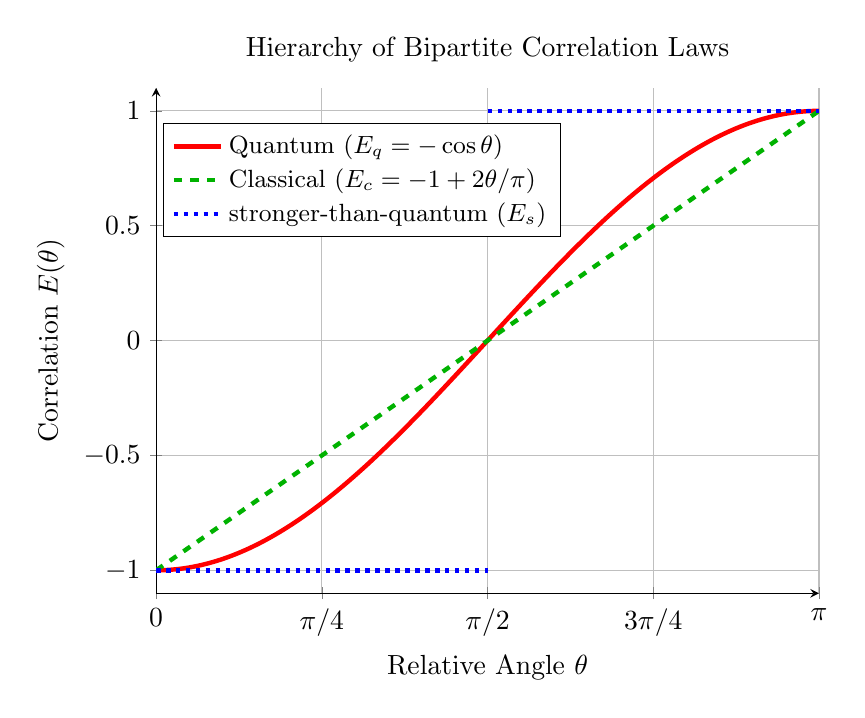
\begin{tikzpicture}
   \begin{axis}[
        title={Hierarchy of Bipartite Correlation Laws},
        xlabel={Relative Angle $\theta$},
        ylabel={Correlation $E(\theta)$},
        xmin=0, xmax=180,
        ymin=-1.1, ymax=1.1,
        axis lines=left,
        xtick={0, 45, 90, 135, 180},
        xticklabels={$0$, $\pi/4$, $\pi/2$, $3\pi/4$, $\pi$},
        ytick={-1, -0.5, 0, 0.5, 1},
        legend style={
            at={(0.01,0.93)},
            anchor=north west,
            font=\small,
        },
        legend cell align={left},
        grid=major,
        width=10cm,
        height=8cm,
    ]

    % 1. Quantum (cosine) correlation
    \addplot[
        domain=0:180,
        samples=200,
        color=red,
        ultra thick,
    ]
    { -cos(x) };
    \addlegendentry{Quantum ($E_q = -\cos\theta$)}

    % 2. Classical (linear) correlation
    \addplot[
        domain=0:180,
        samples=2,
        color=green!70!black,
        dashed,
        ultra thick,
    ]
    { -1 + 2*x/180 };
    \addlegendentry{Classical ($E_c = -1 + 2\theta/\pi$)}

    % 3. stronger-than-quantum (step) correlation
    \addplot[
        domain=0:90,
        samples=2,
        color=blue,
        dotted,
        ultra thick,
    ]
    { -1 };
    \addlegendentry{stronger-than-quantum ($E_s$)}

    \addplot[
        domain=90:180,
        samples=2,
        color=blue,
        dotted,
        ultra thick,
        forget plot
    ]
    { 1 };

    \end{axis}
\end{tikzpicture}
}
    \caption{A comparison of the three correlation functions $E(\theta)$ versus the relative measurement angle $\theta$. The quantum (solid red) and classical (dashed green) correlations only achieve perfect anti-correlation ($E=-1$) at $\theta=0$. The hypothetical stronger-than-quantum correlation (dotted blue) is perfect for any angle $\theta \neq \pi/2$.}
    \label{fig:correlations}
\end{figure}

\subsection{Classical (Linear) Correlation}
A simple local-hidden-variable model~\cite{peres222} gives the linear correlation $E_c(\theta) = -1 + 2\theta/\pi$. To saturate the classical CHSH bound of 2, we choose coplanar angles $\phi_a=2\pi/9$, $\phi_{a'}=-2\pi/9$, $\phi_b=0$, and $\phi_{b'}=4\pi/9$. The relative angles are $\theta_{ab}=\theta_{ab'}=\theta_{a'b}=2\pi/9$ and $\theta_{a'b'}=2\pi/3$. This yields $E_c(2\pi/9) = -5/9$ and $E_c(2\pi/3) = 1/3$, whereby $S_{\mathrm{CHSH}}^{(c)} = |3(-5/9) - 1/3| = 2$.

\subsection{Quantum (Cosine) Correlation}
For a two-qubit singlet state, measurements yield $E_q(\theta) = -\cos\theta$. With the standard CHSH angles $\phi_a=0$, $\phi_{a'}=\pi/2$, $\phi_b=\pi/4$, and $\phi_{b'}=-\pi/4$, the relative angles are $\pi/4$ and $3\pi/4$. The correlations are $E_q(\pi/4)=-\sqrt{2}/2$ and $E_q(3\pi/4)=\sqrt{2}/2$, giving $S_{\mathrm{CHSH}}^{(q)} = 2\sqrt{2}$.

This value, $2\sqrt{2}$, is the maximal allowed in quantum theory. To see this, define the CHSH operator $\mathcal{B} = A\otimes(B+B') + A'\otimes(B-B')$, where $A, A', B, B'$ are Hermitian operators with eigenvalues $\pm1$. Since $A^2=I$, etc., the square of the operator is $\mathcal{B}^2 = 4I\otimes I + [A,A']\otimes[B,B']$. The operator norm is bounded by $\|[X,Y]\| \le 2\|X\|\|Y\|$, so $\|[A,A']\| \le 2$ and $\|[B,B']\| \le 2$. Thus, $\|\mathcal{B}^2\| \le 4+4=8$. It follows that $\|\mathcal{B}\| \le \sqrt{8} = 2\sqrt{2}$, which bounds its expectation value $S_{\mathrm{CHSH}}=|\langle\mathcal{B}\rangle|$ for any quantum state.

\subsection{stronger-than-quantum (Step-Function) Correlation}
A hypothetical no-signaling correlation, stronger than that allowed by quantum mechanics, is the step function~\cite{svozil-krenn,pop-rohr}:
\begin{equation}
E_s(\theta) =\operatorname{sgn}\!\left(\frac{2\theta}{\pi}-1\right)= \begin{cases} -1, & 0\le \theta<\pi/2 \\ +1, & \pi/2<\theta\le\pi \end{cases}
\end{equation}
Using the same angles as in the classical example, $\theta_{ab}$, $\theta_{a'b}$, $\theta_{ab'} < \pi/2$ while $\theta_{a'b'} > \pi/2$. This gives $E_s(2\pi/9)=-1$ and $E_s(2\pi/3)=+1$. The CHSH parameter becomes $S_{\mathrm{CHSH}}^{(s)} = |3(-1) - (+1)| = 4$, saturating the algebraic maximum.

\section{Mutual Information as Thermodynamic Fuel}
The thermodynamic value of these correlations is not given by their degree of nonlocality but by their mutual information. For a joint law $P(x,y|\theta)$, the mutual information is
\begin{equation}
I_\theta(A:E) = \ln 2 - H(A|E) = \ln 2 - h_2\left(\frac{1+E(\theta)}{2}\right),
\label{eq:Itheta}
\end{equation}
where $h_2(p)=-p\ln p-(1-p)\ln(1-p)$ is the binary entropy in nats. This formula is a direct expression of the definition of mutual information, $I(A:E) = H(A) - H(A|E)$. The leading term, $\ln 2$, is the maximal Shannon entropy $H(A)$ for a single unbiased binary system, representing the total initial uncertainty. The binary entropy term, $h_2(\cdot)$, quantifies the conditional entropy $H(A|E)$: the average uncertainty about system A's outcome that \emph{remains} even after the outcome of system E is known. The mutual information is thus the total initial uncertainty reduced by this residual uncertainty, which directly measures the imperfection of the correlation. For a perfect correlation ($E(\theta) = \pm 1$), the conditional entropy is $h_2(0)=h_2(1)=0$, yielding the maximal mutual information $I=\ln 2$. For no correlation ($E(\theta) = 0$), the conditional entropy is maximal at $h_2(1/2)=\ln 2$, yielding zero mutual information. The information content for our three models is:
\begin{align}
I_c(\theta) &= \ln 2 - h_2(\theta/\pi) \\
I_q(\theta) &= \ln 2 - h_2(\sin^2(\theta/2)) \\
I_s(\theta) &= \begin{cases} \ln 2, & \theta\neq \pi/2 \\ 0, & \theta = \pi/2 \end{cases}
\end{align}
In all cases, as depicted in Fig.\ref{fig:mutual_information}, perfect correlation or anti-correlation ($E=\pm 1$) yields the maximal information $I=\ln 2$. Consequently, the maximum work extractable per correlated binary pair, according to Eq.~\eqref{eq:work_from_I}, is universally bounded by $k_{\mathrm{B}}T\ln 2$. While stronger-than-quantum correlations provide maximal mutual information over a wider range of angles, they offer no advantage in the peak extractable work per instance.

\begin{figure}[ht!]
\pgfmathdeclarefunction{h2}{1}{%
  \pgfmathparse{-((#1)==0 ? 0 : (#1)*ln(#1)) - ((1-#1)==0 ? 0 : (1-#1)*ln(1-#1))}%
}
    \centering
    % The user's tikzpicture code is placed directly inside the figure environment
\resizebox{0.4\textwidth}{!}{
    \begin{tikzpicture}
        \begin{axis}[
            %title={Mutual Information for Different Correlation Laws},
            xlabel={Relative Angle $\theta$},
            ylabel={Mutual Information $I(\theta)$ (nats)},
            xmin=0, xmax=180,
            ymin=-0.05, ymax=0.75,
            axis lines=left,
            xtick={0, 45, 90, 135, 180},
            xticklabels={$0$, $\pi/4$, $\pi/2$, $3\pi/4$, $\pi$},
            ytick={0, 0.2, 0.4, 0.6, 0.6931},
            yticklabels={0, 0.2, 0.4, 0.6, $\ln 2$},
            legend style={
                at={(0.5, 0.7)},   % Manually tune here: (0.5, 0.5) is the center
                anchor=center,     % Anchor the legend's center point
                font=\small,       % Use a smaller font
            },
            legend cell align={left},
            grid=major,
            width=11cm,
            height=8cm,
        ]

        % 1. Quantum (cosine) correlation
        \addplot[
            domain=0:180,
            samples=201,
            color=red,
            ultra thick,
            style=solid,
        ]
        { ln(2) - h2( (sin(x/2))^2 ) };
        \addlegendentry{Quantum ($I_q$)}

        % 2. Classical (linear) correlation
        \addplot[
            domain=0:180,
            samples=101,
            color=green!70!black,
            ultra thick,
            style=dashed,
        ]
        { ln(2) - h2(x/180) };
        \addlegendentry{Classical ($I_c$)}

        % 3. stronger-than-quantum (step) correlation
        \addplot[
            domain=0:180,
            samples=2,
            color=blue,
            dotted,
            ultra thick,
        ]
        { ln(2) };
        \addlegendentry{stronger-than-quantum ($I_s$)}

        % Add points for the discontinuity
        \addplot[only marks, mark=*, mark size=3pt, color=blue, fill=white] coordinates {(90, {ln(2)})};
        \addplot[only marks, mark=*, mark size=2pt, color=blue, fill=blue] coordinates {(90, 0)};

        \end{axis}
    \end{tikzpicture}
}
    \caption{Mutual information as a function of relative measurement angle $\theta$ for the three correlation laws discussed in the text: Quantum ($I_q$, solid red), Classical ($I_c$, dashed green), and stronger-than-quantum ($I_s$, dotted blue). While classical and quantum correlations only provide the maximal information resource of $\ln 2$ nats at perfect alignment ($\theta=0$) or anti-alignment ($\theta=\pi$), the hypothetical stronger-than-quantum correlation yields this maximum for all angles except the single point $\theta=\pi/2$.}
    \label{fig:mutual_information}
\end{figure}

\section{Thermodynamic Equivalence versus Operational Robustness}
\label{sec:advantages}
The preceding analysis established that the maximum extractable work from a single bipartite correlation is universally bounded by $k_{\mathrm{B}}T\ln 2$, irrespective of whether the underlying correlation law is classical, quantum, or stronger-than-quantum. This thermodynamic equivalence stems from the fact that all three models can, under ideal conditions, achieve a perfect correlation ($|E(\theta)|=1$) and thus a maximal mutual information of $I(A:E) = \ln 2$.

This perspective, however, obscures significant operational differences in how readily this informational resource can be accessed. The practical advantage of non-classical correlations becomes apparent when one considers the conditions required to achieve this maximum.

\begin{enumerate}
    \item \textbf{Classical Brittleness:} For the classical linear model, $E_c(\theta) = -1 + 2\theta/\pi$, the maximal information is available only at the sharp points $\theta=0$ and $\theta=\pi$. Any deviation from perfect alignment or anti-alignment of the measurement bases results in a linear degradation of the correlation and a corresponding loss of potential work. Accessing the full thermodynamic potential therefore requires a perfectly shared and stable reference frame between the two parties, making the resource \emph{brittle} with respect to experimental noise or misalignment.

    \item \textbf{Quantum Robustness:} The quantum correlation $E_q(\theta) = -\cos\theta$ offers a distinct advantage. While it also requires alignment ($\theta=0$ or $\theta=\pi$) for maximal information, the function's derivative is zero at these points. Consequently, for a small misalignment $\delta\theta$, the deviation from perfect correlation is of order $\mathcal{O}(\delta\theta^2)$. The mutual information near $\theta=0$ is approximately $I_q(\delta\theta) \approx \ln 2 - \mathcal{O}(\delta\theta^2)$, showing a quadratic, rather than linear, decrease. This property makes the quantum resource significantly more \emph{robust} against small experimental imperfections in establishing a shared reference frame.

    \item \textbf{Stronger-Than-Quantum Flexibility:} The hypothetical step-function correlation $E_s(\theta)$ represents the ultimate operational advantage. It yields maximal mutual information ($I_s(\theta) = \ln 2$) for \emph{any} relative angle $\theta \in [0, \pi]$ except for the single measure-zero point at $\theta=\pi/2$. This makes the resource maximally \emph{flexible}. The two parties would not need to coordinate their measurement settings or share a reference frame at all to access the full thermodynamic potential. As long as their chosen bases are not perfectly orthogonal, the correlation is perfect and the maximum work can be extracted.
\end{enumerate}

Thus, a clear operational hierarchy emerges. While the peak thermodynamic value of a single, perfectly established correlation is universal, the practical utility and resilience of that resource are dictated by its nonlocal character. Quantum correlations are operationally superior to classical ones due to their robustness, and hypothetical stronger-than-quantum correlations would be superior still, offering near-total freedom from the physical constraint of a shared reference frame.

\section{Concrete Realization: A Correlation-Powered Engine}
We can illustrate this principle with a modified Szilard engine. The system (A) is a single particle in a box of volume $V$ at temperature $T$. The environment (E) is a distant two-state memory bit. They are prepared in a perfectly correlated state: if E is `0', the particle is in the left half of the box; if E is `1', the particle is in the right half. The initial mutual information is $I_i(A:E) = \ln 2$.

The work extraction cycle is as follows:
\begin{enumerate}
    \item \textbf{Information Acquisition:} An agent measures the memory bit E and finds it in state `0'. This reveals the particle's location without interacting with it.
    \item \textbf{Feedback:} Knowing the particle is on the left, the agent inserts a partition in the middle of the box and places a piston against it. This costs no work.
    \item \textbf{Isothermal Expansion:} The particle expands against the piston, moving it to the right end of the box. The system draws heat from the reservoir to keep its temperature constant, converting it into work.
    \item \textbf{Work Calculation:} The work extracted from this isothermal expansion from $V/2$ to $V$ is:
    \begin{equation}
        W_{\mathrm{ext}} = \int_{V/2}^{V} \frac{k_{\mathrm{B}}T}{v} \,dv = k_{\mathrm{B}}T \ln 2.
        \label{eq:szilard_work}
    \end{equation}
\end{enumerate}
At the cycle's end, the system A has returned to its initial state ($\Delta F_T(\rho_A) = 0$), but the correlation has been consumed ($I_f(A:E) = 0$). The process has converted information worth $k_{\mathrm{B}}T\ln 2$ entirely into work, saturating the bound in Eq.~\eqref{eq:work_from_I}.

\section{Discussion and Conclusion}

Correlations between a system and its environment challenge the classical notion of thermodynamic isolation. Even when energy and matter exchanges are blocked, preexisting correlations allow conditional control and work extraction. These correlations---whether classical, quantum, or stronger-than-quantum---constitute a genuine thermodynamic resource governed by generalized second laws that include information flow.

Our analysis shows that the thermodynamic value of any correlation is universally limited by its mutual information: at most $k_{\mathrm{B}}T\ln 2$ of work can be extracted per perfectly correlated bit, in agreement with Landauer's principle. The apparent hierarchy among classical, quantum and hypothetical superquantum correlations therefore lies not in the magnitude of extractable work but in how robustly that resource can be accessed. Quantum correlations offer a distinct operational advantage, maintaining near-maximal efficiency under small misalignments, whereas classical correlations degrade linearly and superquantum models would be fully alignment-independent.

Recognizing mutual information as the unifying currency of work reconciles thermodynamics and information theory on microscopic scales. Engines that consume correlations do not violate the second law; they reveal that information, too, must be treated as a physical fuel. A truly isolated system must thus be sealed not only against exchanges of energy and matter, but also against preexisting informational ties to its surroundings.

By linking nonlocal correlations to thermodynamic performance, this work clarifies the operational meaning of information in physics and suggests a path toward exploiting quantum correlations as resilient, high-fidelity energy resources in the microscopic domain.

\begin{acknowledgments}
This text was partially created and revised with assistance from one or more of the following large language models: Gemini 2.5 Pro, gpt-5-high.
This research was funded in whole or in part by the  Austrian Science Fund (FWF) Grant DOI: 10.55776/PIN5424624.
The authors acknowledge TU Wien Bibliothek for financial support through its Open Access Funding Programme.
\end{acknowledgments}


\bibliography{svozil}

\end{document}
